%%%%%%%%%%%%%%%%%%%%%%%%%%%%%%%%%%%%%%%%%
% Short Sectioned Assignment
% LaTeX Template
% Version 1.0 (5/5/12)
%
% This template has been downloaded from:
% http://www.LaTeXTemplates.com
%
% Original author:
% Frits Wenneker (http://www.howtotex.com)
%
% License:
% CC BY-NC-SA 3.0 (http://creativecommons.org/licenses/by-nc-sa/3.0/)
%
%%%%%%%%%%%%%%%%%%%%%%%%%%%%%%%%%%%%%%%%%

%----------------------------------------------------------------------------------------
%	PACKAGES AND OTHER DOCUMENT CONFIGURATIONS
%----------------------------------------------------------------------------------------

\documentclass[paper=a4, fontsize=11pt]{scrartcl} % A4 paper and 11pt font size

\usepackage[T1]{fontenc} % Use 8-bit encoding that has 256 glyphs
\usepackage{fourier} % Use the Adobe Utopia font for the document - comment this line to return to the LaTeX default
\usepackage[english]{babel} % English language/hyphenation
\usepackage{amsmath,amsfonts,amsthm} % Math packages

\usepackage{graphicx}

\usepackage{sectsty} % Allows customizing section commands
\allsectionsfont{\centering \normalfont\scshape} % Make all sections centered, the default font and small caps

\usepackage{fancyhdr} % Custom headers and footers
\pagestyle{fancyplain} % Makes all pages in the document conform to the custom headers and footers
\fancyhead{} % No page header - if you want one, create it in the same way as the footers below
\fancyfoot[L]{} % Empty left footer
\fancyfoot[C]{} % Empty center footer
\fancyfoot[R]{\thepage} % Page numbering for right footer
\renewcommand{\headrulewidth}{0pt} % Remove header underlines
\renewcommand{\footrulewidth}{0pt} % Remove footer underlines
\setlength{\headheight}{13.6pt} % Customize the height of the header

\numberwithin{equation}{section} % Number equations within sections (i.e. 1.1, 1.2, 2.1, 2.2 instead of 1, 2, 3, 4)
\numberwithin{figure}{section} % Number figures within sections (i.e. 1.1, 1.2, 2.1, 2.2 instead of 1, 2, 3, 4)
\numberwithin{table}{section} % Number tables within sections (i.e. 1.1, 1.2, 2.1, 2.2 instead of 1, 2, 3, 4)

\setlength\parindent{0pt} % Removes all indentation from paragraphs - comment this line for an assignment with lots of text

%----------------------------------------------------------------------------------------
%	TITLE SECTION
%----------------------------------------------------------------------------------------

\newcommand{\horrule}[1]{\rule{\linewidth}{#1}} % Create horizontal rule command with 1 argument of height

\title{	
\normalfont \normalsize 
\textsc{BRSU} \\ [25pt] % Your university, school and/or department name(s)
\horrule{0.5pt} \\[0.4cm] % Thin top horizontal rule
\huge Homework for Artificial Intelligence for Robotics - Assignment 3 \\ % The assignment title
\horrule{2pt} \\[0.5cm] % Thick bottom horizontal rule
}

\author{Bastian Lang} % Your name

\date{\normalsize\today} % Today's date or a custom date

\begin{document}

\maketitle % Print the title

\section{Theoretical Part}
\subsection{Exercise 1}
\emph{Does a finite state space always lead to a finite search tree? Can you be more precise about
what types of state spaces always lead to finite search trees? (Adapted from Bender, 1996.)}\\\\

No, a finite search space does not always lead to a finite search tree. If there would be bidirectional connections between two states, then the resulting search tree would be infinite. Say for example state A could reach state B and vice versa. The search tree would have state B as a child of state A and state A as a child of state B. So there is an infinite loop.\\
If the finite state space does only have unidirectional connections between states and there is no path from any state to itself using however many states in between, then this will always result in a finite search tree. 

\section{Practical Part}
\subsection{Task Overview}
In this exercise we have been given three text files representing maps.
Each map contains characters which can be interpreted as follows:
\begin{itemize}
\item * $\rightarrow$ Dirt
\item space $\rightarrow$ Empty Space
\item s $\rightarrow$ Robot Starting Position
\item Any other character $\rightarrow$ Obstacle
\end{itemize}
The task was to construct an algorithm that reads the map and uses Breadth-First Search (\emph{BFS}) and Depth-First Search \emph{DFS}) to plan a path for a robot to explore and find each dirt cell.
The rules were given with:
\begin{itemize}
\item The robot can move from one cell to another at each step.
\item The robot can only move to the left, right, up or down cells from the current position.
\item The robot does not have previous knowledge about the environment, such as dirt
positions or obstacles. It has to "explore".
\item The robot cannot move through obstacles and the map is closed.
\end{itemize}
In the end Breath-First Search and Depth-First Search should be compared and for each map 
should be said which algorithm works better based on observed data.

\subsection{Approach}
I started by Dividing the task into a set of small problems. These are
\begin{itemize}
\item read a map file and store the map in an appropriate data structure
\item localize the start position of the robot
\item compute the four possible next positions (four neighbours)
\item filter visited positions and positions already in list
\item choose next action using breadth-first approach
\item choose next action using depth-first approach
\item create algorithm that uses breadth-first or depth-first
\item keep track of maximum nodes stored and number of steps taken
\item print out a map and results
\end{itemize}
Plain naive \emph{BFS} or \emph{DFS} does not care if a node already has been visited. So for this task it was important to not expand nodes that already have been expanded or have already  been stored for future expanding. When expanding a node and adding its children to the queue or stack (depending on BSF or DFS), I only stored those nodes that have not been expanded before (I keep track of those nodes in a separate list) and those nodes who are not already stored in the queue or stack.\\
The robot cannot move through obstacles, therefore a neighbour representing an obstacle will not be added to the explore-list.

\subsection{Results}
\textbf{General remark}: In my implementation I marked the positions the robot has visited so far using small circles. Files containing every single step can be found in the provided resource/results folder.

\subsubsection{Map 1}
For map 1 using BFS the robot needs to explore 1261 positions until the map is clean. It stores 27 nodes at once in its exploration map (and 1261 of course in the list of visited nodes)(see figure \ref{fig:map1_bfs}).\\\\
Using DFS the robot needs to explore 1168 positions and stores 506 nodes at once (see figure \ref{fig:map1_dfs}).\\\\
Comparing both results the DFS completes cleaning the map about 100 steps faster, but needs to store roughly 480 nodes more at the same time, which is about 20 times as much.\\

\begin{figure}[Ht]
	\centering
  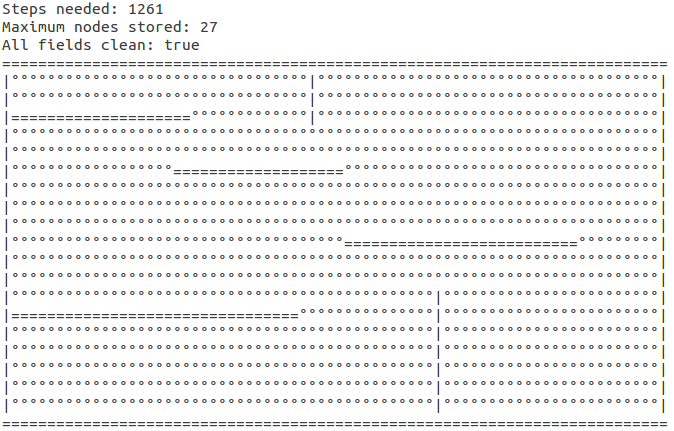
\includegraphics[width=1\textwidth]{images/map1_bfs.png}
	\caption{Result of map1 using BFS}
	\label{fig:map1_bfs}
\end{figure}

\begin{figure}[Ht]
	\centering
  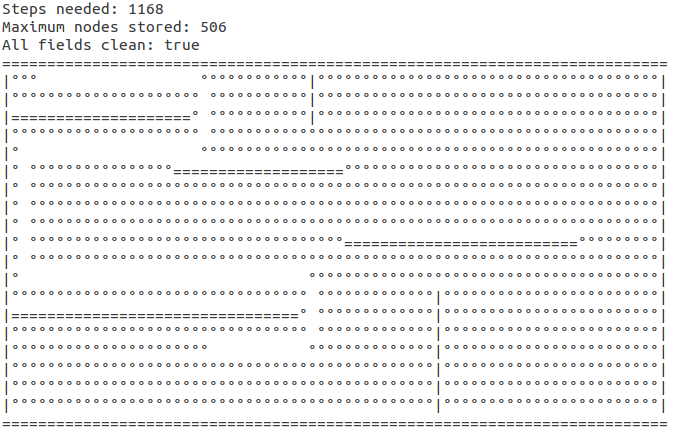
\includegraphics[width=1\textwidth]{images/map1_dfs.png}
	\caption{Result of map1 using DFS}
	\label{fig:map1_dfs}
\end{figure}
 
\subsubsection{Map 2}
For map 2 BFS takes 1073 steps and has to store 20 nodes at the same time (see figure \ref{fig:map2_bfs}).\\\\
DFS needs 1078 steps, but has to store 466 nodes (see figure \ref{fig:map2_dfs}).\\\\
The two algorithms need about the same number of steps, but DFS needs to store about 23 times more nodes.\\

\begin{figure}[Ht]
	\centering
  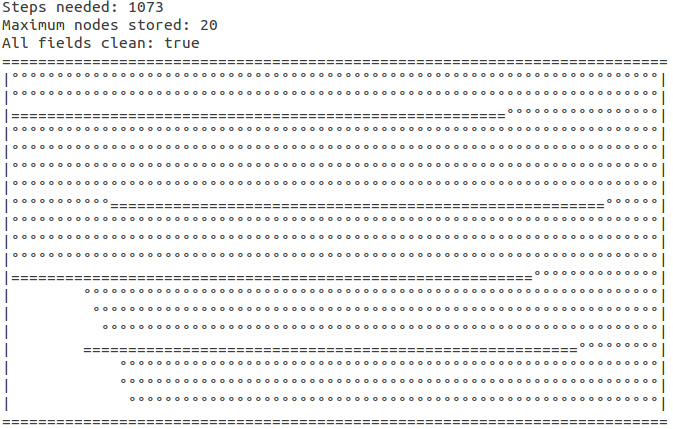
\includegraphics[width=1\textwidth]{images/map2_bfs.png}
	\caption{Result of map2 using BFS}
	\label{fig:map2_bfs}
\end{figure}


\begin{figure}[Ht]
	\centering
  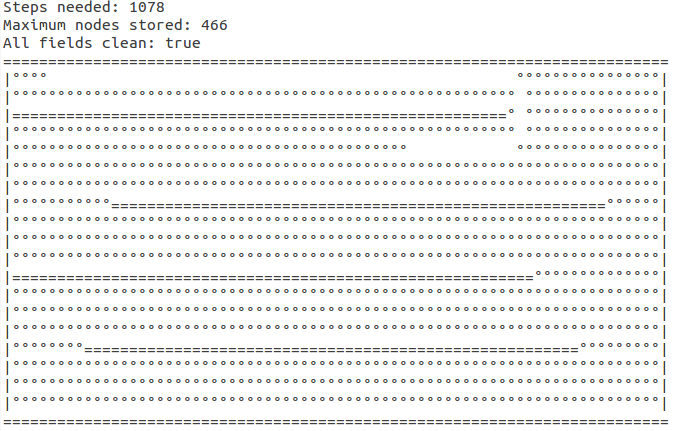
\includegraphics[width=1\textwidth]{images/map2_dfs.png}
	\caption{Result of map2 using DFS}
	\label{fig:map2_dfs}
\end{figure}

\subsubsection{Map 3}
For map 3 BFS takes 2460 steps and has to store 44 nodes at the same time. It is not able to reach and clean all fields in the map (see figure \ref{fig:map3_bfs}).\\\\
DFS cannot reach all of the fields as well and therefore also needs 2460 steps, but has to store up to 878 nodes at once (see figure \ref{fig:map3_dfs}).\\\\
This time again DFS needs to store about 20 times the amount of nodes than BFS. Both algorithms fail to clean the whole map.\\
\begin{figure}[Ht]
	\centering
  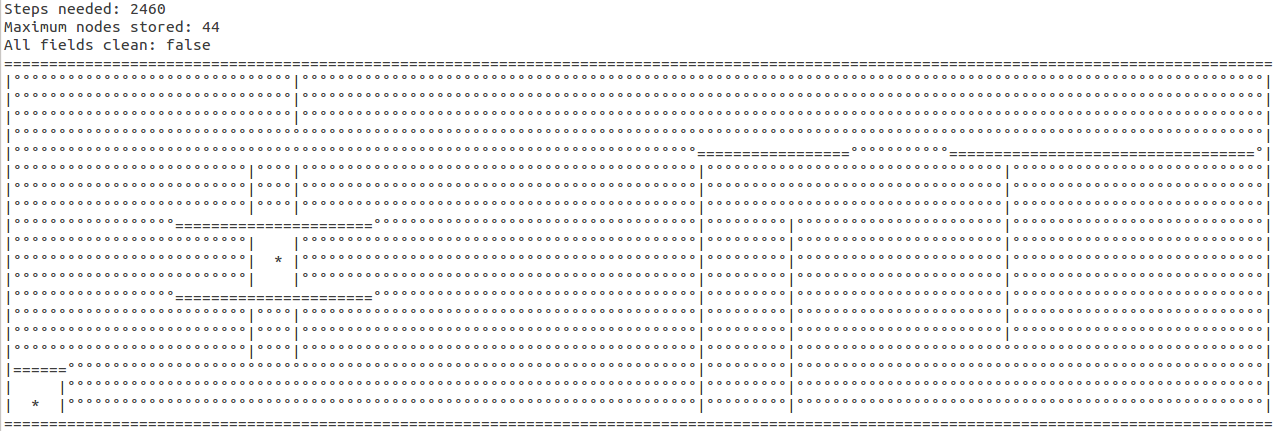
\includegraphics[width=1\textwidth]{images/map3_bfs.png}
	\caption{Result of map3 using BFS}
	\label{fig:map3_bfs}
\end{figure}

\begin{figure}[Ht]
	\centering
  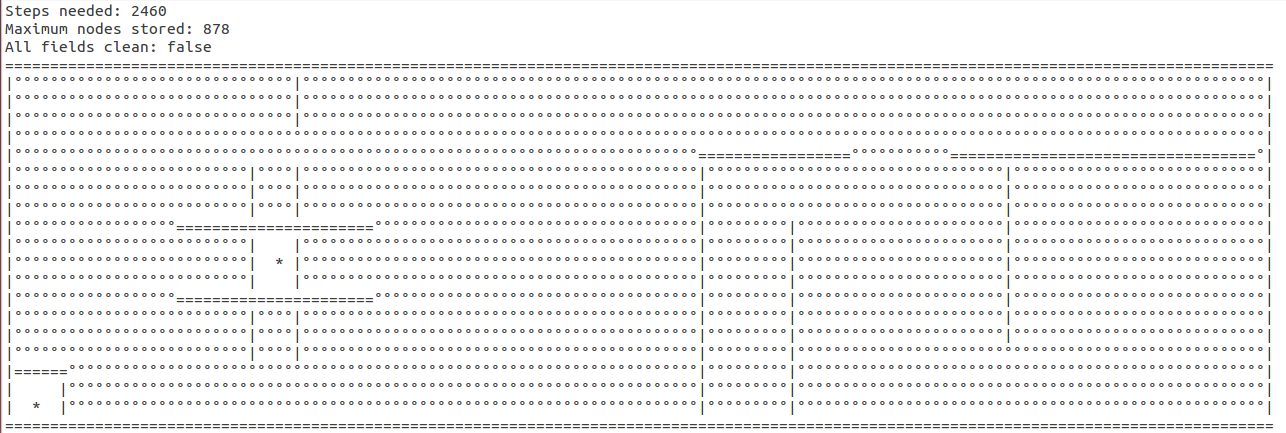
\includegraphics[width=1\textwidth]{images/map3_dfs.png}
	\caption{Result of map3 using DFS}
	\label{fig:map3_dfs}
\end{figure}

\subsubsection{Conclusion}
Both algorithms are complete. They find a solution if one exists. Both are not optimal because they do not find the optimal solution.\\
The time complexity of DFS for the first map is about 8\% better. But for all the maps BFS has the better space complexity.\\\\
For my architecture and the given maps neither the time advantage for map 1 of DFS nor the space advantage in all maps for BFS are significant enough to clearly favour one algorithm over the other as for both are complete. But thinking about way bigger problems the BFS approach is the one to go with.\\
Both algorithms have to look for the child nodes of every node in their list of nodes to expand. So having a list 20 times bigger will result in much more computation time for DFS.

\end{document}